\chapter{Prewrite}
\label{cha:prewrite}

\section{Result 01}
\label{sec:-02}

\begin{theorem}[Model 01: connected]
	\label{thm:-01}
	Let \( \Omega \coloneqq \{(x^\prime, x_n) \text{ s.t. }\lvert x^\prime \rvert \leq
	1,\lvert x_n \rvert \leq M \} \) and \( E_0 \coloneqq \{ (x^\prime,x_n) \text{ s.t. }
	\lvert x^\prime \rvert \leq R, \lvert x_n \rvert \geq M \} \) for some \( R, M > 0 \).
	Then there exists an \( M_0 \) s.t.\ for all \( M \leq M_0 \) the minimizer of the
	fractional perimeter is connected and given by \( E_M = \Omega \cup E_0 \).
\end{theorem}

\begin{figure}[h]
	\centering
	\def\svgwidth{0.4\textwidth}
	\import{figures}{model01.pdf_tex}
	\caption{Model 01}
	\label{fig:-03}
\end{figure}

\begin{proof}
	Proof by contradiction. Assume \( E_M \) is not \( E_0 \cup \Omega \), then we can
	slide a ball of radius \( r \) down and at some point it will touch \( E_M \). We
	consider the ball \( B_r (t e_n) \). Since \( E_M \) not cylindrical, there exists \(
	r_0 \in (0,1) \) and \( t_0 > 0 \) s.t.\ \( \partial B_{r_0}(t_0 e_n) \cap \partial
	E_M \neq \emptyset \) and \( B_{r_0}(t e_n) \subset E_M \) for all \( t > t_0 \). \\
	Since \( E_M \) is a minimizer it is also a variational solution and the inequality
	holds
	\[
		\int_{\mathbb{R}^n} \frac{\chi_{E_M^c}(y)-\chi_{E_M} (y)}{\lvert y-q\rvert^{n+s}} \dd{y} \geq 0
	\]
	whereas \( q \in \partial B_{r_0}(t_0 e_n) \cap \partial E_M \). \\
	We show that the left hand side is negative. Split the domain into four parts, as seen
	in the Figure:
	\begin{figure}[h]
		\centering
		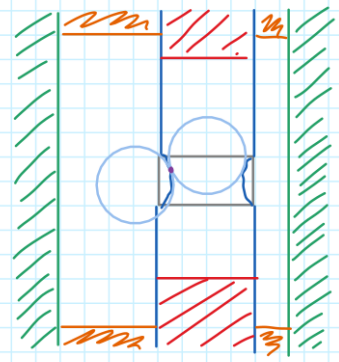
\includegraphics[width = 0.5\textwidth]{figures/Screenshot_20240105_020915.png}
		\caption{}
		\label{fig:-01}
	\end{figure}
	\par
	We define
	\begin{align*}
		A                                & \coloneqq \{ (x^\prime,x_n) \text{ s.t. } \lvert x^\prime -q^\prime \rvert \geq R+1\} \text{ Green Area} \\
		B                                & \coloneqq \{ (x^\prime,x_n) \text{ s.t. } \lvert x^\prime \rvert < R, \lvert x_n -q_n \rvert > 2M \} \\
		C                                & \coloneqq \{ (x^\prime,x_n) \text{ s.t. } \lvert x^\prime \rvert \geq R, \lvert x^\prime - q^\prime \rvert \leq R+1, \lvert x_n -q_n \rvert > \Lambda M \} \\
		\text{Everything else} \subset S & \coloneqq \{(x^\prime,x_n) \text{ s.t. } \lvert x^\prime -q^\prime \rvert \leq R+1, \lvert x_n -q_n \rvert \leq \Lambda M \}
	\end{align*}


	Integration over the first part:
	\begin{gather*}
		\int_A \frac{\chi_{E^c} -\chi_E}{\lvert y-q\rvert^{n+s}} \dd{y} \overset{A \subset E^c}{ =} \int_{ \lvert y^\prime \rvert > R+1} \frac{1}{\lvert y \rvert^{n+s}} \dd{y} \leq c(n) \int_{R+1}^\infty r^{-s-2} \dd{y} \leq c(n,s) R^{-(1+s)}
	\end{gather*}

	Integration over the second part:
	\begin{gather*}
		\int_B \frac{\chi_{E^c} -\chi_E}{\lvert y-q \rvert^{n+s}} \dd{y} \overset{B \subset E}{ =} - \int_B \frac{1}{\lvert y-q\rvert^{n+s}} \dd{y} \leq -c(n,s) M^{-s} \qquad \text{Idea: Consider ball with factor \( 2^{-n} \)}
	\end{gather*}

	Integration over the third part:
	\begin{align*}
		 & \int_C \frac{\chi_{E^c} -\chi_E}{\lvert y-q\rvert^{n+s}} \dd{y} \overset{C \subset E^C}{ =} \int_C \frac{1}{\lvert y-q\rvert^{n+s}} \dd{y} \leq c(n) \int_{R-1}^{R+1} \int_{\Lambda M}^\infty \frac{r^{n-2}}{(r^2 +y_n^2)^{\frac{n+s}{2}}} \dd{y_n} \dd{r} \\
		 & \overset{r^2 \leq r^{2 + y_n^2}}{ \leq} c(n) \int_{R-1}^{R+1} \int_{2
		\Lambda M}^\infty \frac{1}{(r^2 +y_n^2)^{\frac{s+2}{2}}} \dd{y_n} \dd{r} \overset{\text{convexity}}{\leq} \int_{R-1}^{R+1} \int_{\Lambda M}^\infty \frac{1}{(r+y_n)^{s+2}} \dd{y_n} \dd{r} \\
		 & \leq c(n,s) \int_{R-1}^{R+1} \frac{1}{(r+\Lambda M)^{s+1}} \leq c(n,s)(R-1+\Lambda M)^{-s} \leq c(n,s)(\Lambda M)^{-s}
	\end{align*}

	Integration over the fourth part: \\
	Justifiction that we can estimate with \( S \): Only negative part of the integration
	is fully in the set we want to estimate and the rest in \( S \) is positive. \\
	We split \( S \) into four parts:
	\begin{enumerate}[label = \roman*)]
		\item \( S \cap B_{\Lambda M} (q) \cap B_{r_0}(z) \)
		\item \( S \cap B_{\Lambda M} (q) \cap B_{r_0}( \overline{z}) \)
		\item \( S \cap (B_{\Lambda M} (q)\setminus ( B_{r_0}(z) \cup
		      B_{r_0}(\overline{z}))) \)
		\item \( S \setminus B_{\Lambda M} (q) \)
	\end{enumerate}
	where \( \overline{z}\coloneqq z + 2(q-z) \) and \( \Lambda > 4 \) chosen big enough
	and \( M \) chosen small enough s.t.\ \( \Lambda M \leq 1 \). \\
	We estimate the first and second part:
	\begin{align*}
		     & \int_{S \cap B_{\Lambda M} (q) \cap B_{r_0}(z) \cup S \cap B_{\Lambda M} (q) \cap B_{r_0}(\overline{z})} \frac{\chi_{E^c}- \chi_E}{\lvert y-q\rvert^{n+s}} \dd{y} \\
		\leq & \int_{S \cap B_{\Lambda M} (q) \cap B_{r_0}(z)} \frac{1}{\lvert y-q\rvert^{n+s}} \dd{y} - \int_{S \cap B_{\Lambda M} (q) \cap B_{r_0}(\overline{z})} \frac{1}{\lvert y-q\rvert^{n+s}} \dd{y} \leq 0
	\end{align*}
	These two intgerals cancel because of symmetry. \\
	We estimate the third part:
	\begin{gather*}
		\int_{S \cap (B_{\Lambda M} (q)\setminus ( B_{r_0}(z) \cup B_{r_0}(z)))}\frac{\chi_{E^c}- \chi_E}{\lvert y-q\rvert^{n+s}} \dd{y} \leq \int_{P_{1,\Lambda M}} \frac{1}{\lvert y-q\rvert^{n+s}} \dd{y} \leq C \Lambda^{1-s} M^{1-s}
	\end{gather*}
	where we used lemma 3.1 in 2016 dipierro-savin-valdinoci with \( R = r_0 = 1 and
	\lambda = \Lambda M \) (we can choose \( r_0 = 1 \), since if we can show the bound
	for \( r_0 = 1 \) then it holds for all smaller balls as well). \\
	We estimate the fourth part:
	\begin{gather*}
		\int_{S\setminus B_{\Lambda M} (q)} \frac{\chi_{E^c}- \chi_E}{\lvert y-q\rvert^{n+s}} \dd{y} \leq \int_{B_{R+2}\setminus B_{\Lambda M}} \frac{1}{\lvert y\rvert^{n+s}} \dd{y} = c(n,s)((\Lambda M)^{-s} - (R+2)^{-s})
	\end{gather*}
	since \( S \subset B_{R+2} \) for \( R \geq 1 \) since \( ((\Lambda M)^2 +
	(R+1)^2)^{\frac{1}{2}} \leq (R^2 + 4R+4)^{\frac{1}{2}} = R+2 \). \\
	\par
	Thus in total we get:
	\begin{align*}
		\int_{\mathbb{R}^n} \frac{\chi_{E^c}- \chi_E}{\lvert y-q\rvert^{n+s}} \dd{y}
		 & \leq -c_1 M^{-s} + c_0 (R^{-(1+s)} + (\Lambda M)^{-s} + (\Lambda M)^{-s} - (R+2)^{-s} + \Lambda^{1-s} M^{1-s}) \\
		 & \leq -c_1 M^{-s}(1- + \frac{c_0}{c_1} (R^{-(1+s)}M^s + 2 \Lambda^{-s} -(R+2)^{-s} M^s + \Lambda^{1-s} M
		\intertext{Choose \( \Lambda \) large and \( M \) small enoguh}
		 & \leq -c_2 M^{-s} < 0
	\end{align*}
\end{proof}


\section{Result 02}
\label{sec:-03}

\begin{theorem}[Model 01: disconnected]
	\label{thm:-02}
	Let the setting be as in theorem \cref{thm:-01}, then there exists an \( M_0 \) s.t.\
	for all \( M \geq M_0 \) the minimizer of the fractional perimeter is disconnected.
\end{theorem}
\begin{proof}
	Proof analogous to theorem 1.2 in 2016 dipierro-onoue-valdinoci. \\
\end{proof}

\section{Result 03}
\label{sec:-04}

\begin{theorem}[Model 02: connected]
	\label{thm:-03}
	Let \( \Omega \coloneqq \{(x^\prime, x_n) \text{ s.t. } \lvert x^\prime \rvert \leq 1,
	\lvert x_n \rvert \leq M \} \) and \( E_0 \coloneqq \{ (x^\prime, x_n) \text{ s.t. } M
	\leq \lvert x_n \rvert \leq R+M \} \). For every \( R > 0 \) there exists a \( M_0 \)
	s.t.\ for all \( M \leq M_0 \) the minimizer of the fractional perimeter is connected.
	(We need \( R > M \))
\end{theorem}
\begin{note}
	To prove this we need to show that minimizers are always connected to \( \Omega^c \)
	and i.e.\ \( d(E_0, \Omega) = d(E\setminus E_0, \Omega) \).
\end{note}
\begin{proof}
	We show that for every \( R > 0 \) at least the tube \( \{ \lvert x_n \rvert < r_0 \}
	\) is in the minimizer for some \( r_0 > 0 \). \\
	We do that analogously to theorem \cref{thm:-01} by contradiction. We assume that \(
	E_M \) is disconnected, thus we can slide a ball of radius \( r \) down and for all \(
	r_0 \in (0,1) \) there exists a \( t_0 > 0 \) s.t.\ \( \partial B_{r_0}(t_0 e_n) \cap
	\partial E_M \neq \emptyset \). If we can show that there exists a \( r_0 \) s.t.\
	this conntradicts then the tube is in the minimizer. It is enough to show that for one
	\( r_0 \) since if we can contradict this for one \( r_0 \) then for all smaller there
	is no touching as well. \\
	For that we split into four parts as seen in the figure:
	\begin{figure}[h]
		\centering
		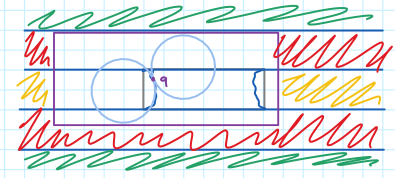
\includegraphics[width = 0.8\textwidth]{figures/Screenshot_20240107_160324.png}
		\caption{}
		\label{fig:-02}
	\end{figure}
	\par
	We define
	\begin{align*}
		A & \coloneqq \{(x^\prime,x_n) \text{ s.t. } \lvert x_n \rvert \geq M+R \} \\
		B & \coloneqq \{(x^\prime,x_n) \text{ s.t. } \lvert x_n \rvert \leq M, \lvert x^\prime -q^\prime \rvert > 2 \} \\
		C & \coloneqq E_0 \setminus S \\
		S & \coloneqq \{ (x^\prime,x_n) \text{ s.t. } \lvert x_n - q_n \rvert \leq M+R, \lvert x^\prime -q^\prime \rvert \leq 2\}
	\end{align*}

	Integration over the first part:
	\begin{align*}
		     & \int_A \frac{\chi_{E^c} -\chi_E}{\lvert y-q\rvert^{n+s}} \dd{y} \overset{A \subset E^c}{ \leq} \int_{\lvert y_n \rvert \geq R} \frac{1}{\lvert y \rvert^{n+s}} \dd{y} \leq c(n) \int_0^\infty \int_R^\infty \frac{r^{n-2}}{(r^2 +y_n^2)^{\frac{n+s}{2}}} \dd{y_n} \dd{r} \\
		\leq & \ c(n) \int_0^\infty \int_R^\infty \frac{1}{(r^2 +y_n^2)^{\frac{s+2}{2}}} \dd{y_n} \dd{r} \leq c(n) \int_0^\infty \int_R^\infty \frac{1}{(r+y_n)^{s+2}} \dd{y_n} \dd{r} \\
		=    & \ c(n,s) \int_0^\infty \frac{1}{(r+R)^{s+1}} \dd{r} = c(n,s) R^{-s}
	\end{align*}

	Integration over the second part:
	\begin{align*}
		     & \int_B \frac{\chi_{E^c} -\chi_E}{\lvert y-q\rvert^{n+s}} \dd{y} \overset{B \subset E^c}{ \leq} c(n) \int_0^M \int_2^\infty \frac{r^{n-2}}{(r^2 +y_n^2)^{\frac{n+s}{2}}} \dd{r} \dd{y_n} \\
		\leq & \ c(n) \int_0^M \int_2^\infty \frac{1}{( r+y_n)^{s+2}} \dd{r} \dd{y_n} = c(n,s) \int_0^M \frac{1}{(2+y_n)^{s+1}} \dd{r} \\
		=    & \ c(n,s)(2^{-s}-(2+M)^{-s}) \leq c(n,s) 2^{-s}
	\end{align*}

	Integration over the third part (here we need \( R > M \)):
	\begin{align*}
		\int_C \frac{\chi_{E^c} -\chi_E}{\lvert y-q\rvert^{n+s}} \dd{y} = - \int_C \frac{1}{\lvert y-q \rvert^{n+s}} \dd{y} \leq -c(n) \int_{B_M (\ldots)} \frac{1}{\lvert y\rvert^{n+s}} \dd{y} \leq -c(n,s) M^{-s}
	\end{align*}
	Idea: Move part of the stripe outside, restrict to ball with radius \( M \) and
	multiply with \( \frac{1}{2} \) since not whole ball may be in the set.\\

	Integration over the fourth part: \\
	We split \( S \) into four parts:
	\begin{enumerate}[label = \roman*)]
		\item \( S \cap B_{\Lambda M} (q) \cap B_{r_0}(z) \)
		\item \( S \cap B_{\Lambda M} (q) \cap B_{r_0}( \overline{z}) \)
		\item \( S \cap (B_{\Lambda M} (q)\setminus ( B_{r_0}(z) \cup B_{r_0}(z))) \)
		\item \( S \setminus B_{\Lambda M} (q) \)
	\end{enumerate}
	where \( \overline{z}\coloneqq z + 2(q-z) \) and \( \Lambda > 4 \) chosen big enough
	and \( M \) chosen small enough s.t.\ \( \Lambda M \leq 1 \). \\
	Again the first and second part are in sum smaller than zero. \\
	We estimate the third part:
	\begin{align*}
		     & \int_{S \cap (B_{\Lambda M} (q)\setminus ( B_{r_0}(z) \cup B_{r_0}(\overline{z})))} \frac{\chi_{E^c} -\chi_E}{\lvert y-q\rvert^{n+s}} \dd{y} \\
		\leq & \ \int_{P_{r_0, 1}} \frac{1}{\lvert y\rvert^{n+s}} \dd{y} + \int_{B_{\Lambda M}\setminus B_{r_0}} \frac{1}{\lvert y\rvert^{n+s}} \dd{y} \leq c(n,s) (r_0^{-s} - (\Lambda M)^{-s})
	\end{align*}
	We estimate the fourth part:
	\begin{align*}
		     & \int_{S \setminus B_{\Lambda M}(q)} \frac{\chi_{E^c} -\chi_E}{\lvert y-q\rvert^{n+s}} \dd{y} \\
		\leq & \ c(n) \int_{\Lambda M}^{R+3} \frac{1}{r^{s+1}} \dd{r} \leq c(n,s)((\Lambda M)^{-s} - (R+3)^{-s})
	\end{align*}
	Thus we estimate the domain \( S \) with
	\begin{align*}
		\int_S \frac{\chi_{E^c} -\chi_E}{\lvert y-q\rvert^{n+s}} \dd{y} \leq c(n,s)(r_0^{-s} - (R+3)^{-s}) \leq c(n,s) r_0^{-s}
	\end{align*}
	\par
	Thus in total we get:
	\begin{align*}
		\int_{\mathbb{R}^n} \frac{\chi_{E^c} -\chi_E}{\lvert y-q\rvert^{n+s}} \dd{y}
		 & \leq -c_0 M^{-s} +c_1 (R^{-s}+2^{-s} + r_0^{-s}) \\
		 & \leq -c_0 M^{-s}(1- \frac{c_1}{c_0} (R^{-s}M^s + 2^{-s}M^s + r_0^{-s}M^s))
		\intertext{Now choose \( r_0 = \frac{R}{2} \) and at most \( 2 \)}
		 & \leq -c_0 M^{-s}(1- \frac{c_1}{c_0} (R^{-s}M^s + 2^{-s}M^s + \left(\frac{2M}{R}\right)^s))
		\intertext{Choose \( \Lambda \) large and \( M \) small enoguh}
		 & \leq -c_2 M^{-s} < 0
	\end{align*}
\end{proof}

\section{Result 04}
\label{sec:-05}

\begin{theorem}[Model 02: disconnected]
	\label{thm:-04}
	Let the setting be as in theorem \cref{thm:-03}, then there exists an \( M_0 \) s.t.\
	for all \( M \geq M_0 \) the minimizer of the fractional perimeter is disconnected.
\end{theorem}
\begin{proof}
	Proof analogous to theorem 1.2 in 2016 dipierro-onoue-valdinoci. (I think) \\
\end{proof}

\section{Result 05}
\label{sec:-06}

